\documentclass[10pt,twocolumn,letterpaper]{article}

\usepackage{cvpr}
\usepackage{times}
\usepackage{epsfig}
\usepackage{graphicx}
\usepackage{amsmath}
\usepackage{amssymb}
\usepackage{float}

% Include other packages here, before hyperref.

% If you comment hyperref and then uncomment it, you should delete
% egpaper.aux before re-running latex.  (Or just hit 'q' on the first latex
% run, let it finish, and you should be clear).
\usepackage[breaklinks=true,bookmarks=false]{hyperref}

\cvprfinalcopy % *** Uncomment this line for the final submission

\def\cvprPaperID{****} % *** Enter the CVPR Paper ID here
\def\httilde{\mbox{\tt\raisebox{-.5ex}{\symbol{126}}}}

% Pages are numbered in submission mode, and unnumbered in camera-ready
%\ifcvprfinal\pagestyle{empty}\fi
\providecommand{\tightlist}{%
  \setlength{\itemsep}{0pt}\setlength{\parskip}{0pt}}
\setcounter{page}{1}
\begin{document}

%%%%%%%%% TITLE
\title{Modern methods of Detecting DDoS attacks in SDN}

\author{B. Sujeeth Kumar\\
\href{mailto:es19btech11022@iith.ac.in}{es19btech11022@iith.ac.in}
% For a paper whose authors are all at the same institution,
% omit the following lines up until the closing ``}''.
% Additional authors and addresses can be added with ``\and'',
% just like the second author.
% To save space, use either the email address or home page, not both
\and
G. Sai Sidhardha\\
\href{mailto:cs19btech11050@iith.ac.in}{cs19btech11050@iith.ac.in}
\and
Krishn V. Kher\\
\href{mailto:es19btech11015@iith.ac.in}{es19btech11015@iith.ac.in}
\and
M. Bharat Chandra\\
\href{mailto:es19btech11016@iith.ac.in}{es19btech11016@iith.ac.in}
\and
M. Sri Akhil\\
\href{mailto:es19btech11014@iith.ac.in}{es19btech11014@iith.ac.in}
}

\maketitle
%\thispagestyle{empty}

%%%%%%%%% ABSTRACT
\begin{abstract}
% Discuss what our project is on
In this project, we attempt to develop a prototype framework that efficiently detects DDoS intrusions in real time networks based on modern Deep Learning based methods. We also try to go one step further and explore certain existing implementations for preventing/mitigating certain kinds of DDoS attacks. Finally we also present a new idea (to the best of our knowledge) for converting resource-targeting DDoS attacks to bandwidth-targeting DDoS attacks, so that the prevention/mitigation procedures applied for bandwidth-targeting DDoS attacks can be applied to resource-targeting DDoS attacks as well.
\end{abstract}

%%%%%%%%% BODY TEXT
\section{Introduction}
The Internet has become a large part of our lives ever since it came in existence, in the late 20th century. Ever since, thousands and millions of improvised Internet-based communication systems have been proposed, tested and deployed in real time. Many protocols have been proposed and deployed even upon existing network infrastructures. Both hardware and software based ideas have been proposed for improvement on various Internet-based services. 
\\
\par However, the downside is that despite all these successes, there were also many problems that we have been encountering. Some have got solved elegantly, some have been partially solved or have been solved for specific systems, while there are still many issues that remain unsolved. 
\\
\par One of the major concerns in the last category is the problem of secure communications and services. There is so much importance and variety associated with the domain of network security that there are even whole academic degrees and jobs offered just in the domain of Cryptography and Network Security!
\\
\par Looking back 40-50 years, we have evolved a lot in this domain; we have defined a whole mathematical framework to define threat models and develop (possibly) complex and secure protocols that provide the service even under those adversarial conditions. This is what is usually studied in Cryptography.
A major part of Networking Security involves extending the theoretical threat scenarios studied in Cryptography, in real time and exploring safe and efficient models accordingly. \textbf{Now in Networking Security, an attack on a real time client-server kind of system is informally defined as some sort of a malicious attempt to hamper the intended services of the server or any sort of communications between the genuine client and server}. 
\\
\par There are many, many kinds of attacks that have been discovered, since the time the Internet was deployed. Precautionary measures and mitigation strategies have been devised for many of them, but unfortunately there are still many attacks that have no complete anti-attack solution. One may (rightly) wonder on the fact that 

Part of the reason why this is so because some security problems are inherently hard and it is a major challenge to actually devise protocols that only defend from an attacker while also providing legitimate services to genuine users. 
Another observation is that the fact that the large number of security vulnerabilities still present in today's systems seems to indicate that the application of secure protocols and practices in real systems seems to be going at a much slower paces than the corresponding advances in theoretical Cryptographic research. 
Part of the reason for this is that when the Internet was initially designed, many of the resulting protocols and services were designed keeping in mind non-malicious users. However, unfortunately, within a matter of a decade it was observed that this assumption was not true! 

One such domain of attacks that we concentrate on in this paper is \textit{DoS} attacks. DoS stands for Denial-of-Service. Informally stated, attacks under this domain try to overload the server and/or its resources in some way or the underlying network routing the packets between the client and server, thus making it unable to render legitimate services to genuine users. There is a subdomain of DoS attacks known as \textit{DDoS} attacks. DDoS stands for Distributed-Denial-of-Service. Attacks under this domain try to achieve the goal of DoS attacks, in a distributed manner, i.e. they try to employ various network nodes and machines to overwhelm the target server/system.

In the recent times of COVID-19, the number of DDoS attack has unfortunately been on the rise as can be seen in Fig.1. 
    \begin{figure}[h]
    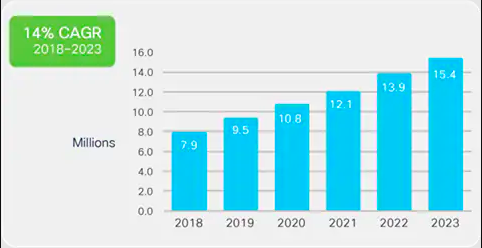
\includegraphics[width = 0.45\textwidth]{src/img/ddos_cisco.png}
    \caption{Source: Cisco Annual Report}
    \label{fig:incep}
    \end{figure}
Even as recently as January-February 2022, a huge spike was observed in the number of DDoS attacks in certain parts of the globe due to various reasons. Due to such attacks certain important/sensitive websites were down for extended periods of time, causing much financial and social damage {ref: Fig.2}.
    \begin{figure}[h]
    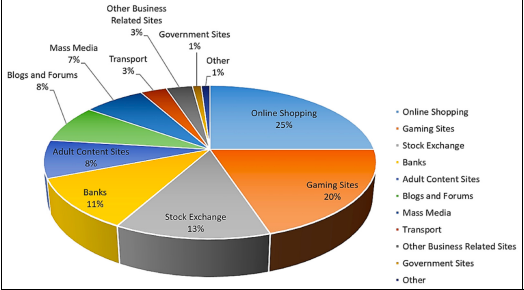
\includegraphics[width = 0.45\textwidth]{src/img/ddos_pie.png}
    \caption{Breakdown of attacked sites in Q2 2011 \cite{ddos_survey}}
    \label{fig:incep}
    \end{figure}
According to a research report published by the \href{https://www.ponemon.org/}{Ponemon Institute} in 2012, the average cost incurs for 1 minute downtime as a result of DDoS attacks was approximately US \$22,000 which may range from US \$1 to US \$100,000. These sort of unwanted discrepancies motivate the strong and urgent need to come up with solutions which can defend against DDoS attacks.

We are focusing on trying to detect and mitigate DDoS attacks in a SDN based networking. SDN based networking has become a popular trend, especially ever since the paper that proposed it \cite{sdn}.
\section{Literature Review}

There are many DDoS detection and prevention measures currently available. This survey paper \cite{ddos_survey} gives a very detailed report on most of the existing DDoS attacks and the common prevention/mitigation methods currently existing.

Before the age of classical Machine Learning, DDoS attacks used to usually get detected by monitors that would keep on collecting the statistics. Then either a network administrator had to keep an eye on the nature of the statistics, to have any chance of detecting a DDoS attack before it was actually launched.

Things changed for the better after classical ML models were researched upon \cite{ml_survey}. However with the rise of Deep Learning based methods and their success in image recognition, speech models, semantic text understandings, etc., researchers have started trying DL based approaches to learn the functions and thresholds from various datasets to detect DDoS attacks \cite{ddos1} \cite{ddos2}.

\section{Proposed methodology}
We first discuss the detection approaches we tried to explore as a part of this project. Later on, we also present the relevant accuracy and efficiency metrics which various models gave.
We then discuss our attempts on mitigating and propose a possibly novel idea (proof of concept design) for mitigation. 
\subsection{System Design}
Below is the pictorial representation for our system's design.
\begin{figure}[h]
    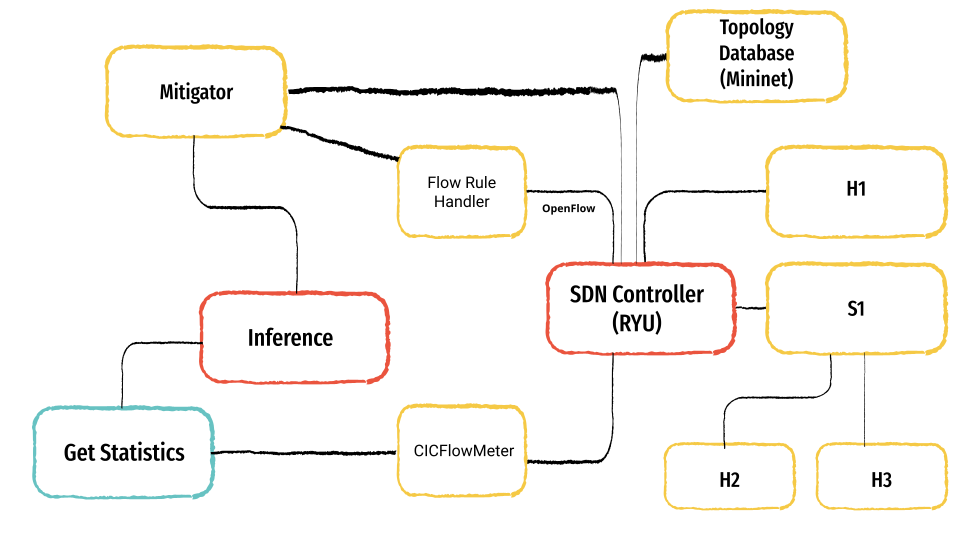
\includegraphics[width = 0.45\textwidth]{src/img/system_design.png}
    \caption{System Design}
    \label{fig:incep}
\end{figure}
\href{https://public.flourish.studio/visualisation/9782692/}{Here }is an interactive representation of the same for better understanding


\subsection{Detection}

We used supervised and semi-supervised learning based approaches. We also used ensemble methods under supervised learning based approaches. These models classify test samples derived from feature extractor of the SDN framework.

% Tell that we used supervised and unsupervised learning. Then describe the models, their architectures.
% Keep an image for input and output clusterings via t-SNE.

\subsubsection{Supervised Learning}

\begin{itemsize}
\tightlist
    \item \textbf{Multi-Layer-Perceptron}:
    We implemented a deep learning model more specifically an autoencoder attached to a layer which predicts whether there is an attack or not and also classifies it according to the type of DDoS attack {ref: <link>}. The reason we used autoencoder is because of the fact that the autoencoder can significantly increase the anomaly detection accuracy compared to linear and kernel Principal Component Analysis. It also helps in getting a compact representation of the input data flow. Finally the compact representation of the data is passed onto a \texit{softmax} layer to predict the type of DDoS attack.\\\\
    \par The model receives a 77 dimension vector as input is connected to a FCC (fully connected layer) to give 64 dimensions. It is then reduced to 32,16,8. This is the encoder structure of the model. This is then followed by a decoder which reconstructs the 64 dimensions in the exact reverse manner. All the layers use ReLU  activation function. The output from the decoder is then sent to a FCC to give out an 8 dimensional vector(since we are only classifying 8 types of DDoS attacks) and a softmax activation is done on it to predict the classes.\\\\
    The loss function is a simple categorical cross entropy loss between the output labels and the true labels.\\
    \par We also tried to use some machine learning models to do the inference and they performed very well compared to the deep learning models.\\\\
    \item \textbf{CatBoost}:
    CatBoost is based on gradient boosted decision trees. During training, a set of decision trees is built consecutively. Each successive tree is built with reduced loss compared to the previous trees. The number of trees is controlled by the starting parameters.We used this model since it is an extremely efficient ensemble method which does very well in classifying large data.\\
     \item \textbf{LGBM classifier}:
     LightGBM is a gradient boosting framework based on decision trees to increase the efficiency of the model and reduce memory usage. It uses two novel techniques: Gradient-based One Side Sampling and Exclusive Feature Bundling which fulfills the limitations of histogram-based algorithm that is primarily used in all Gradient Boosting Decision Tree frameworks.
\end{itemsize}

\subsubsection{Semi-Supervised Learning}


\begin{itemsize}
\tightlist
    \item \textbf{Variational Auto Encoder}:
    A variational autoencoder (VAE) provides a probabilistic manner for describing an observation in latent space. Thus, rather than building an encoder which outputs a single value to describe each latent state attribute, it formulates an encoder to describe a probability distribution for each latent attribute. Our hope was that it define a distribution for each type of attack and then classify the type of attack.\\
    The architecture is shown in Figure 3, where it has an encoder and decoder portion (unsupervised learning) followed by a final classifier MLP architecture (supervised learning) to classify the data.\\
    The loss functions used were a combination of categorical cross entropy for reconstruction loss (unsupervised portion), KL divergence loss and categorical cross entropy loss for the classification loss(supervised portion).\\
    \begin{figure}[h]
    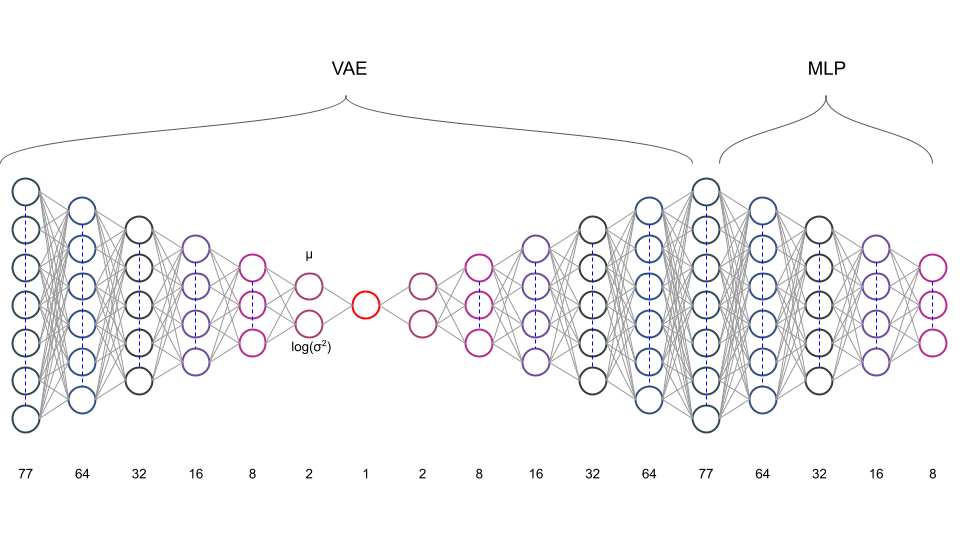
\includegraphics[width = 0.45\textwidth]{src/img/vae.png}
    \caption{VAE Architecture}
    \label{fig:incep}
\end{figure}
\end{itemsize}


\subsection{Prevention/Mitigation} % See which one do we actually do. also the mycielski thing maybe

\section{Implementation}
The following modules have been implemented:
\begin{enumerate}
\itemsep-0.81em
  \item Network Topology
  \item Ryu Application
  \item Deep Learning and Machine Learning models
\end{enumerate}
\par The network topology has been implemented using the "Mininet" package. 
For preliminary testing, a simple linear topology (keep image), with 1 switch, 3 hosts and 1 controller, has been implemented.
\par The SDN controller has been implemented using the Ryu API. The SDN controller populates the flow rules in the switches and performs flow classification in real time.
\par The deep learning and machine learning models have been trained independently and saved in pickle files. The pickle files are loaded in the SDN controller to perform inference.
\par A DDoS attack is generated from one of the hosts to another host belonging to the same subnet. The "Hyenae" utility has been used for this purpose. Since packets flow through the switches, packets are captured at the switch interfaces using the "tshark" utility and are saved in a pcap file. The "cicflowmeter" utility has been used to read the pcap file to generate the features into a csv file.
\par The features are extracted in the SDN controller and the inference is done.

\subsection{Feature Extractor (FE)}
% tell how we collect features. basically use cicflowmeter i think (implementation)


\subsection{Traffic Classifier (TC)}
% explain a bit on the classification part (implementation)

\subsection{Response on Alert (RoA)}

\section{Evaluation \& Results}

\subsection{Model Training}

\subsection{Dataset}
% Talk about data pre-processing. Also tell about public/private dataset thing. Maybe also show a picture of what features are considered important, as is shown in XGBoost, CatBoost.

\subsection{Accuracy \& Efficiency}
Here we show the accuracies of various models so that we could pick the best model for the DDoS detection. 

\subsubsection{Auto Encoder Model Statistics}
The statistics of the Auto Encoder Model can be seen in the below graphs.\\
The validation accuracy we obtained was \textbf{0.8143}
\begin{figure}[h]
    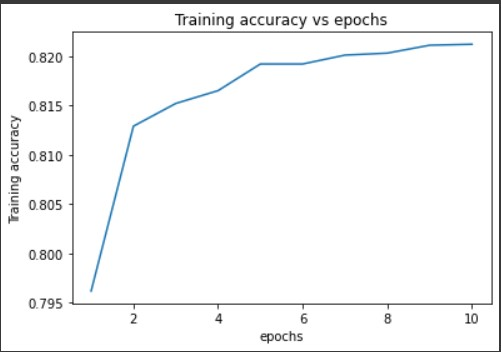
\includegraphics[width = 0.45\textwidth]{src/img/graphs/an_acc.jpg}
    \caption{The Auto Encoders training accuracy vs epochs}
    \label{fig:incep}
\end{figure}

\begin{figure}[h]
    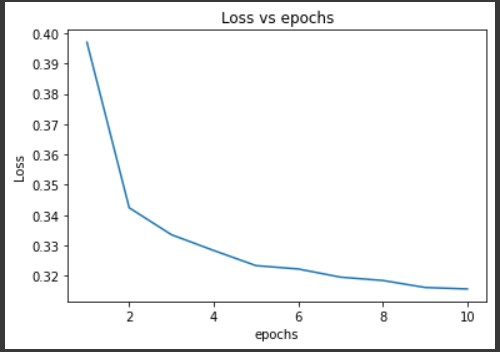
\includegraphics[width = 0.45\textwidth]{src/img/graphs/an_loss.jpg}
    \caption{The Auto Encoders Loss vs epochs}
    \label{fig:incep}
\end{figure}

\begin{figure}[h]
    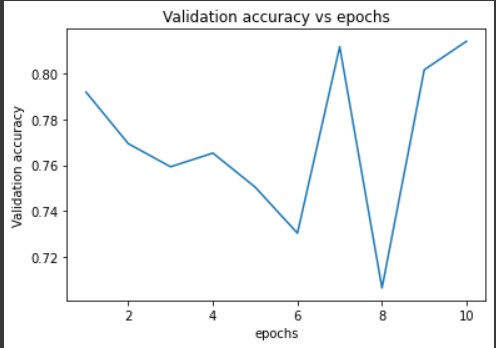
\includegraphics[width = 0.45\textwidth]{src/img/graphs/an_val_acc.jpg}
    \caption{The Variational Auto Encoders validation accuracy vs epochs}
    \label{fig:incep}
\end{figure}
\subsubsection{CatBoost Classifier Statistics}
The confusion matrix of the CatBoost Classifier Model on validation data can be seen in the below graphs.\\
The validation accuracy we obtained was \textbf{0.8642051139521957}
\begin{figure}[h]
    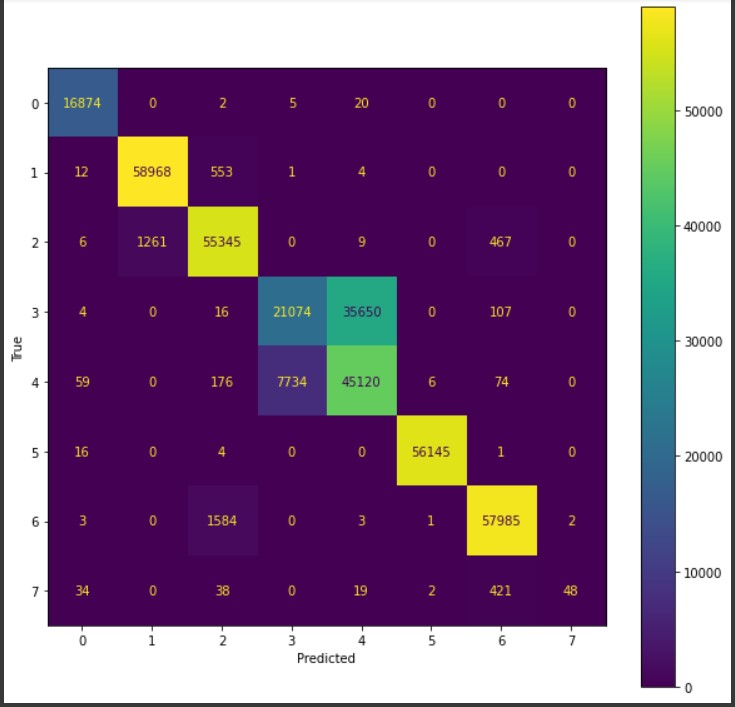
\includegraphics[width = 0.45\textwidth]{src/img/results/cat_cm.jpg}
    \caption{The CatBoost confusion matrix}
    \label{fig:incep}
\end{figure}

\subsubsection{LGBM Classifier Statistics}
The confusion matrix of the LGBM Classifier Model on validation data can be seen in the below graphs.\\
The validation accuracy we obtained was \textbf{0.8700441569196311}
\begin{figure}[h]
    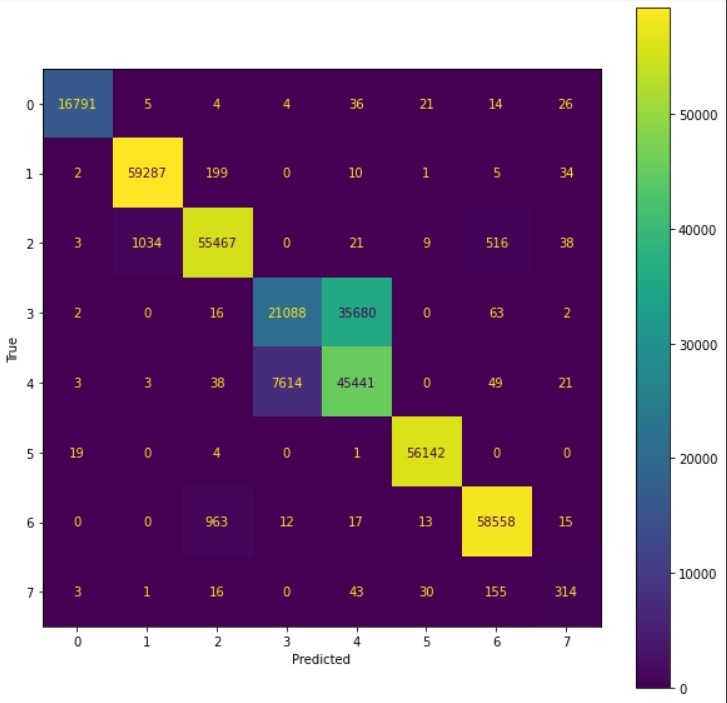
\includegraphics[width = 0.45\textwidth]{src/img/results/lg_cm.jpg}
    \caption{The LGBM confusion matrix}
    \label{fig:incep}
\end{figure}

\subsubsection{Variational Auto Encoder Model Statistics}
The statistics of the Variational Auto Encoder Model can be seen in the below graphs.\\
The validation accuracy we obtained was \textbf{0.6840}
\begin{figure}[h]
    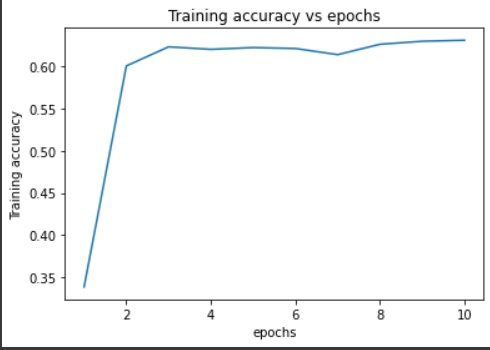
\includegraphics[width = 0.45\textwidth]{src/img/graphs/vae_acc.jpg}
    \caption{The Variational Auto Encoders training accuracy vs epochs}
    \label{fig:incep}
\end{figure}

\begin{figure}[h]
    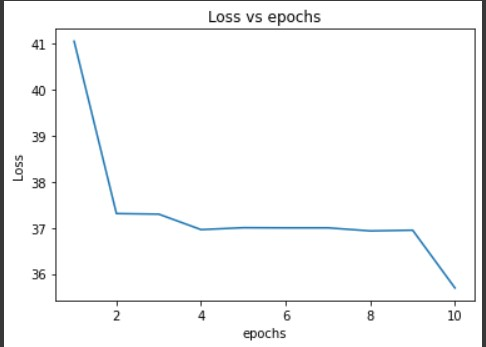
\includegraphics[width = 0.45\textwidth]{src/img/graphs/vae_loss.jpg}
    \caption{The Variational Auto Encoders Loss vs epochs}
    \label{fig:incep}
\end{figure}

\begin{figure}[h]
    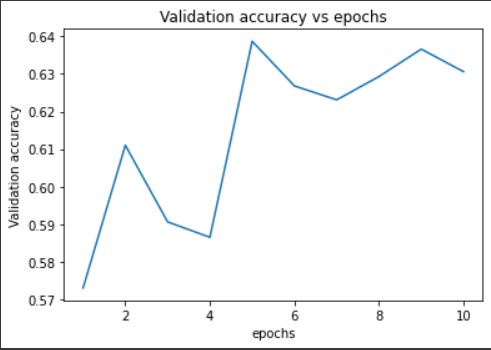
\includegraphics[width = 0.45\textwidth]{src/img/graphs/vae_val_acc.jpg}
    \caption{The Variational Auto Encoders validation accuracy vs epochs}
    \label{fig:incep}
\end{figure}

\begin{figure}[h]
    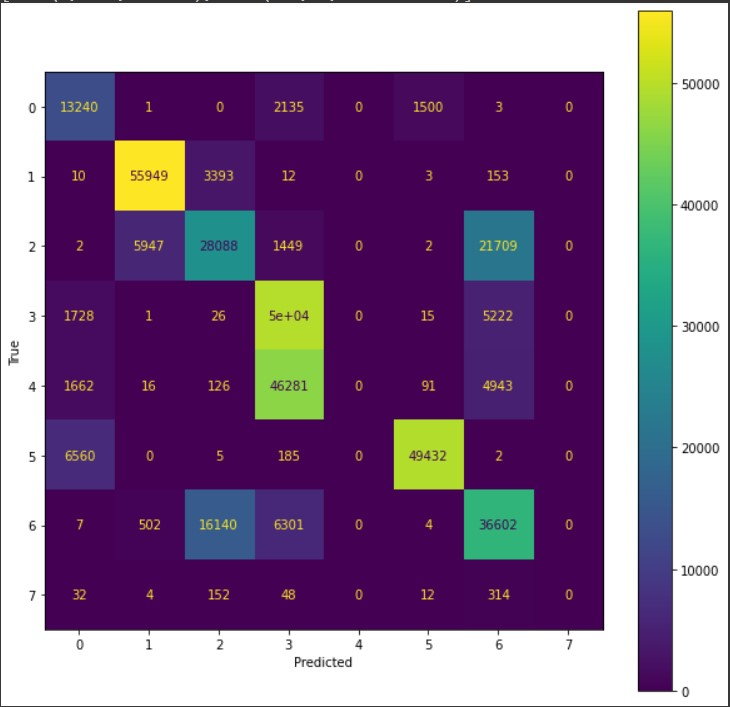
\includegraphics[width = 0.45\textwidth]{src/img/results/vae_cm.jpg}
    \caption{The VAE confusion matrix}
    \label{fig:incep}
\end{figure}
% Talk about the accuracy metrics (precision matrix, f1, roc whatever for all models). Show time vs epochs, loss vs. time and other such plots.

\subsection{Attack Simulation} % Talk about the Hyenae thing and all. how we arrange the botnet. show pictures.

\subsection{Model Inference}
 % talk about how different models respond in real time, accuracy wise and how efficient they are. some plots too i guess. 
 % preferably for each model maybe, we'll see
 
 % Quote papers against whom we beat accuracy also I guess, preferably Tahir ji's paper :)
 
\subsection{Prevention/Mitigation efficacy}
% does the p/m strategy really work


\section{Conclusions and Future Scope}
% What could we conclude and how could we have improved it, suggestions.

\section{Acknowledgement} % any other miscellaneous stuff??
We would like to thank Mr.Tahir Ahmed Shaik\cite{capsaeul} \href{mailto:cs20mtech14007@iith.ac.in}{cs20mtech14007@iith.ac.in} for his valuable help in providing us insights on training strategies and deployment of various tools for this project. We thank Dr. Kotaro Kataoka on explaining us different aspects of networking required for the project and also for giving us alternatives when we were stuck at some stages of the project.  



{\small
\bibliographystyle{ieee_fullname}
\bibliography{egbib}
}

\end{document}
